\documentclass[journal,12pt,twocolumn]{IEEEtran}

\usepackage{enumitem}
\usepackage{amsmath}
\usepackage{siunitx}
\usepackage{circuitikz}
\usepackage{amssymb}
\usepackage{gensymb}
\usepackage{graphicx}
\usepackage{txfonts}         
\usepackage{listings}
\usepackage{lstautogobble}
\usepackage{mathtools}
\usepackage{bm}
\usepackage{tikz}
\usepackage{hyperref}
\usepackage{polynom}
\usepackage{capt-of}
\newcommand{\solution}{\noindent \textbf{Solution: }}
\providecommand{\brak}[1]{\ensuremath{\left(#1\right)}}
\providecommand{\rect}[1]{\text{rect}\ensuremath{\left(#1\right)}}
\providecommand{\cbrak}[1]{\ensuremath{\left\{#1\right\}}}
\providecommand{\sbrak}[1]{\ensuremath{\left[#1\right]}}
\providecommand{\mean}[1]{E\left[ #1 \right]}
\providecommand{\foutranin}[1]{\mathcal{F}\cbrak{#1}}
\providecommand{\foutranfin}[1]{\int_{-\infty}^{\infty}{#1}e^{-j2\pi ft}\,dt}
\providecommand{\sinc}[1]{\text{sinc}\ensuremath{\left(#1\right)}}
\providecommand{\var}[1]{\mathrm{Var}\left[ #1 \right]}
\providecommand{\der}[1]{\mathrm{d} #1}
\providecommand{\gauss}[2]{\mathcal{N}\ensuremath{\left(#1,#2\right)}}
\providecommand{\mbf}{\mathbf}
\providecommand{\abs}[1]{\left\vert#1\right\vert}
\providecommand{\norm}[1]{\left\lVert#1\right\rVert}
\providecommand{\z}[1]{{\mathcal{Z}}\{#1\}}
\providecommand{\ztrans}{\overset{\mathcal{Z}}{ \rightleftharpoons}}
\providecommand{\system}[1]{\overset{\mathcal{#1}}{ \longleftrightarrow}}
\providecommand{\laplaceinv}[1]{{\mathcal{L}^{-1}\ensuremath{\left[#1\right]}}}
\providecommand{\parder}[2]{\frac{\partial}{\partial #2} \brak{#1}}

\let\StandardTheFigure\thefigure
\let\vec\mathbf

\numberwithin{equation}{section}
\renewcommand{\thefigure}{\theenumi}
\renewcommand\thesection{\arabic{section}}

\newcommand{\myvec}[1]{\ensuremath{\begin{pmatrix}#1\end{pmatrix}}}
\newcommand{\mydet}[1]{\ensuremath{\begin{vmatrix}#1\end{vmatrix}}}
\newcommand{\define}{\stackrel{\triangle}{=}}

\DeclareMathOperator*{\argmin}{arg\,min}
\DeclareMathOperator*{\argmax}{arg\,max}


\lstset {
	frame=single, 
	breaklines=true,
	columns=fullflexible,
	autogobble=true
}             
   


\begin{document}
                             
\title{ Digital Signal Processing \\ \Large EE3900: Linear Systems and Signal Processing \\ \large Indian Institute of Technology Hyderabad \\ \vspace*{12pt} \textbf{Fourier Series}}
\author{Lokesh Badisa\\ \normalsize AI21BTECH11005 \\ \vspace*{20pt} \normalsize 12 Oct 2022  }
 \maketitle 
 \tableofcontents
 \begin{abstract}
    This manual provides a simple introduction to Fourier Series
    \end{abstract}
    \section{Periodic Function}
    Let 
    \begin{align}
        x(t) &= A_0\abs{\sin\brak{2\pi f_0 t}}
        \label{eq:10-orig-diff-def}
    \end{align}
    \begin{enumerate}[label=\thesection.\arabic*
    ,ref=\thesection.\theenumi]
    \item Plot $x(t)$.\\
    \solution 
    \begin{lstlisting}
        wget https://raw.githubusercontent.com/LokeshBadisa/EE3900-Linear-Systems-and-Signal-Processing/main/charger/codes/1.1.py
        python3 1.1.py
    \end{lstlisting}
    \begin{figure}[!ht]
			\centering
			\includegraphics[width=\columnwidth]{./figs/1.1}
			\caption{}
			%\label{fig:ckt}
\end{figure}
    \item Show that $x(t)$ is periodic and find its period.
    \solution 
    If a signal $x(t)$ is periodic then
    \begin{align}
    x(t+T)=x(t)
    \end{align}
    where $T$ is known as fundamental period.
    \indent Since $|sin\theta|$ function is periodic, x(t) is also periodic.
    \begin{align}
\text{Fundamental Period}=T=\frac{1}{2}\brak{\frac{2 \pi}{2 \pi f_0}}\\
\label{eq:ftp}
=\frac{1}{2f_0}
    \end{align}
    \end{enumerate}
    \section{Fourier Series}
    Consider $A_0 =12$ and $f_0 = 50$ for all numerical calculations.
    \begin{enumerate}[label=\thesection.\arabic*,ref=\thesection.\theenumi]
    \item If
    %\cite{proakis_dsp}
    \begin{align}
        x(t) = \sum_{k = -\infty}^{\infty}c_ke^{\j2\pi kf_0 t}
    \label{eq:one-Z-complex}
    \end{align}
    show that 
    \begin{align}
        c_k = f_0\int_{-\frac{1}{2f_0}}^{\frac{1}{2f_0}}x(t)e^{-\j2\pi kf_0 t}\, dt
    \label{eq:one-Z}
    \end{align}
    \solution 
    From \eqref{eq:one-Z-complex},
    \begin{align}
            x(t) = \sum_{k = -\infty}^{\infty}c_ke^{\j2\pi kf_0 t}
    \end{align}
    Mulitply $e^{-\j2\pi lf_0 t}$ on both sides
    \begin{align}
    x(t)e^{-\j2\pi lf_0 t}=\sum_{k = -\infty}^{\infty}c_ke^{\j2\pi kf_0 t}e^{-\j2\pi lf_0 t}
    \end{align}
    Integrate on both sides with respect to 't' between $-T$ to $T$ where T is fundamental time period of x(t).\\
    Using \eqref{eq:ftp},
    \begin{align}
    T=\frac{1}{2f_0}
    \end{align}
    \begin{align}
    \int_{-\frac{1}{2f_0}}^{\frac{1}{2f_0}}x(t)e^{-\j2\pi kf_0 t}\, dt=\int_{-\frac{1}{2f_0}}^{\frac{1}{2f_0}}\sum_{k = -\infty}^{\infty}c_ke^{\j2\pi \brak{k-l}f_0 t}\,dt\\
    =\sum_{k = -\infty}^{\infty}c_k\int_{-\frac{1}{2f_0}}^{\frac{1}{2f_0}}e^{\j2\pi \brak{k-l}f_0 t}\,dt
    \end{align}
    The above integral:
    \begin{align}
    \int_{-\frac{1}{2f_0}}^{\frac{1}{2f_0}}e^{\j2\pi \brak{k-l}f_0 t}\,dt=
          \begin{cases}
0 & k\neq l
\\
 \int_{-\frac{1}{2f_0}}^{\frac{1}{2f_0}}1\,dt& k=l
\end{cases}
    \end{align}
    \begin{align}
   \therefore \int_{-\frac{1}{2f_0}}^{\frac{1}{2f_0}}x(t)e^{-\j2\pi kf_0 t}\, dt &=\brak{\frac{1}{f_0}}c_k\\
  \therefore c_k = f_0\int_{-\frac{1}{2f_0}}^{\frac{1}{2f_0}}x(t)e^{-\j2\pi kf_0 t}\, dt
    \end{align}
        \item Find $c_k$ for 
        \eqref{eq:10-orig-diff-def}\\
        \solution
        $c_k$ can be calculated even simpler by using
        \begin{align}
        c_k = 2f_0\int_{0}^{\frac{1}{2f_0}}x(t)e^{- \j2 \pi kf_0 t}\, dt
        \end{align}
        $x(t)=A_0 \sin\brak{2 \pi f_0t}$ in 0 to $\frac{1}{2f_0}$ region.\\
Also,
        \begin{align}
        \label{eq:sin}
     \sin \theta  =\frac{e^{\j\theta}-e^{-\j \theta}}{2\j} 
      \end{align}
      Using \eqref{eq:sin},
      \begin{align}
      c_k &= 2f_0\int_{0}^{\frac{1}{2f_0}}A_0 \brak{\frac{e^{\j2\pi f_0t}-e^{-\j 2\pi f_0t}}{2\j}} e^{- \j2 \pi kf_0 t}\,dt\\
      &=A_0f_0\int_{0}^{\frac{1}{2f_0}} \brak{\frac{e^{\j2\pi\brak{1-k} f_0t}-e^{\j 2\pi\brak{-1-k} f_0t}}{\j}}\,dt\\
&=A_0f_0\sbrak{\frac{e^{\j2\pi\brak{1-k} f_0t}}{-2\pi \brak{1-k}f_0}\Big|_0^{\frac{1}{2f_0}} - \frac{e^{\j2\pi\brak{-1-k} f_0t}}{-2\pi \brak{-1-k}f_0}\Big|_0^{\frac{1}{2f_0}}}\\
&=A_0\sbrak{\frac{e^{j\pi\brak{1-k}}-1}{2\pi\brak{k-1}}-\frac{e^{-j\pi\brak{1+k}}-1}{2\pi\brak{k+1}}}
      \end{align}
      \begin{equation}
      \label{eq:ck}
     = \begin{cases}
\frac{2A_0}{\pi\brak{1-k^2}}&k=even
\\
0&k=odd
\end{cases}
      \end{equation}
    \item Verify 
        \eqref{eq:10-orig-diff-def}
        using python.\\
        \solution 
        \begin{lstlisting}
        wget https://raw.githubusercontent.com/LokeshBadisa/EE3900-Linear-Systems-and-Signal-Processing/main/charger/codes/2.3.py
        python3 2.3.py
        \end{lstlisting}
          \begin{figure}[!ht]
			\centering
			\includegraphics[width=\columnwidth]{./figs/2.3}
			\caption{}
			%\label{fig:ckt}
\end{figure}
         \item Show that 
    \begin{align}
        x(t) = \sum_{k = 0}^{\infty}\brak{a_k\cos{2\pi kf_0 t}+b_k\sin{2\pi kf_0 t}}
    \label{eq:one-Z-real}
    \end{align}
    and obtain the formulae for $a_k$ and $b_k$.\\
    \solution
    Using \eqref{eq:one-Z-complex},
    \begin{align}
    x(t) = \sum_{k = -\infty}^{\infty}c_ke^{\j2\pi kf_0 t}
    \end{align}
    As,
    \begin{align}
    e^{\j2\pi kf_0 t}=\cos\brak{2\pi kf_0 t}+j\sin\brak{2\pi kf_0 t}
    \end{align}
    Substituting leads to
    \begin{align}
    x(t) &= \sum_{k = -\infty}^{\infty}c_k\sbrak{\cos\brak{2\pi kf_0 t}+j\sin\brak{2\pi kf_0 t}}\\
    \label{eq:2.4}
    &=\sum_{k = -\infty}^{\infty}c_k\cos\brak{2\pi kf_0 t}+jc_k\sin\brak{2\pi kf_0 t}\\
    &=\sum_{k = -\infty}^{-1}\sbrak{c_k\cos\brak{2\pi kf_0 t}+jc_k\sin\brak{2\pi kf_0 t}}+c_0+\sum_{k = 1}^{\infty}\sbrak{c_k\cos\brak{2\pi kf_0 t}+jc_k\sin\brak{2\pi kf_0 t}}\\
    &=\sum_{k = 1}^{\infty}\sbrak{c_{-k}\cos\brak{2\pi kf_0 t}-jc_{-k}\sin\brak{2\pi kf_0 t}}+c_0+\sum_{k = 1}^{\infty}\sbrak{c_k\cos\brak{2\pi kf_0 t}+jc_k\sin\brak{2\pi kf_0 t}}\\
    &=c_0+\sum_{k = 1}^{\infty}\sbrak{\brak{c_k+c_{-k}}\cos\brak{2\pi kf_0 t}+j\brak{c_k-c_{-k}}\sin\brak{2\pi kf_0 t}}
    \end{align}
    Replacing $\brak{c_k+c_{-k}}\to a_k$ and $j\brak{c_k-c_{-k}} \to b_k$,
    \begin{align}
&=c_0+    \sum_{k = 1}^{\infty}\brak{a_k\cos{2\pi kf_0 t}+b_k\sin{2\pi kf_0 t}}\\
&=\sum_{k = 0}^{\infty}\brak{a_k\cos{2\pi kf_0 t}+b_k\sin{2\pi kf_0 t}}
    \end{align}
    \begin{align}
    \label{eq:u1}
    \therefore a_k=
    \begin{cases}
    c_k+c_{-k}&k\neq0
    \\
    c_0&k=0
    \end{cases}\\
    \label{eq:u2}
    b_k=j\brak{c_k-c_{-k}}
    \end{align}
    Using \eqref{eq:one-Z},
    \begin{align}
    c_k = f_0\int_{-\frac{1}{2f_0}}^{\frac{1}{2f_0}}x(t)e^{-\j2\pi kf_0 t}\, dt\\
    c_{-k} = f_0\int_{-\frac{1}{2f_0}}^{\frac{1}{2f_0}}x(t)e^{\j2\pi kf_0 t}\, dt\end{align}
    \begin{align}
    a_k=c_k+c_{-k}&= f_0\int_{-\frac{1}{2f_0}}^{\frac{1}{2f_0}}x(t)\sbrak{e^{-\j2\pi kf_0 t}+e^{\j2\pi kf_0 t}}\, dt\\
    &=2f_0\int_{-\frac{1}{2f_0}}^{\frac{1}{2f_0}}x(t)\cos\brak{2\pi kf_0t}\, dt
    \end{align}
    Parallely,
    \begin{align}
    b_k&=-2jf_0\int_{-\frac{1}{2f_0}}^{\frac{1}{2f_0}}x(t)\sin\brak{2\pi kf_0t}\, dt
    \end{align}
    \item Find $a_k$ and $b_k$ for 
        \eqref{eq:10-orig-diff-def}\\
        \solution
        Using \eqref{eq:u1} and \eqref{eq:u2} with \eqref{eq:ck},
    \begin{align}
    a_k=c_k+c_{-k}=\begin{cases}
\frac{4A_0}{\pi\brak{1-k^2}}&k=even
\\
\frac{2A_0}{\pi}&k=0
\\
0&k=odd
\end{cases}\\
b_k=j\brak{c_k-c_{-k}}=0
    \end{align}
    \item Verify 
    \eqref{eq:one-Z-real}
    using python.\\
     \solution 
        \begin{lstlisting}
        wget https://raw.githubusercontent.com/LokeshBadisa/EE3900-Linear-Systems-and-Signal-Processing/main/charger/codes/2.6.py
        python3 2.3.py
        \end{lstlisting}
          \begin{figure}[!ht]
			\centering
			\includegraphics[width=\columnwidth]{./figs/2.6}
			\caption{}
			%\label{fig:ckt}
\end{figure}
    \end{enumerate}
    \section{Fourier Transform}
 
\begin{enumerate}[label=\thesection.\arabic*
,ref=\thesection.\theenumi]
\item 
	\begin{align}
		\delta(t)&=0, \quad t\neq0
\\
		\int_{-\infty}^{\infty}\delta(t) \, dt&= 1
	\end{align}
 \item The Fourier Transform of $g(t)$ is
 \begin{align}
 \label{eq:foutraneq}
 G(f)=\int_{-\infty}^{\infty}g(t)e^{-j2\pi ft}\,dt
 \end{align}
 \item Show that 
 \begin{align}
	 g(t-t_0)&\system{F}G(f)e^{-j2\pi ft_0}\\
 \end{align}
 \solution 
 \begin{align}
 \mathcal{F}\cbrak{g(t-t_0)}=\int_{-\infty}^{\infty}g(t-t_0)e^{-j2\pi ft}\,dt\\
 =e^{-j2\pi ft_0}\int_{-\infty}^{\infty}g(t-t_0)e^{-j2\pi f\brak{t-t_0}}\,dt\\
=G(f)e^{-j2\pi ft_0}
 \end{align}
 \item Show that 
 \begin{align}
 \label{eq:duality}
	 G(t)&\system{F}g(-f)
 \end{align}\\
 \solution From the definition of Inverse Fourier Transform
 \begin{align}
 g(t)=\int_{-\infty}^{\infty}G(f)e^{j2\pi ft}\,df
 \end{align}
 Replace t $\to$ f,
 \begin{align}
  g(f)=\int_{-\infty}^{\infty}G(t)e^{j2\pi ft}\,dt
  \end{align}
  Replace f $\to$ -f,
  \begin{align}
   g(-f)=\int_{-\infty}^{\infty}G(t)e^{-j2\pi ft}\,dt\\
    =\mathcal{F}\cbrak{G(t)}
  \end{align}
  \begin{align}
  \therefore  G(t)&\system{F}g(-f)
 \end{align}
 \item $\delta(t)\system{F}?$\\
 \solution
 \begin{align}
 \foutranin{\delta(t)}=\foutranfin{\delta(t)}\\
 =\int_{-\infty}^{\infty}\delta(t)\,dt\\
 \end{align}
 Since $e^{-j2\pi ft}=1$ for t=0 and remaining integrand is zero for t $\neq0$.
 \begin{align}
  =\int_{-\infty}^{\infty}\delta(t)\,dt\\
  =1
 \end{align}
 \item $e^{-j2\pi f_0t}\system{F}?$\\
 \solution 
 \begin{align}
 \foutranin{e^{-j2\pi f_0t}}=\int_{-\infty}^{\infty}1\cdot e^{-j2\pi\brak{f+f_0}t}\,dt\\
 =\int_{-\infty}^{\infty}\foutranin{\delta(t)} e^{-j2\pi\brak{f+f_0}t}\,dt
 \end{align}
 Using \eqref{eq:duality},
 \begin{align}
 \label{eq:eft}
 =\delta(-(f+f_0))=\delta(f+f_0)
 \end{align}
 \item $\cos(2\pi f_0t)\system{F}?$\\
 \solution
 \begin{align}
 \foutranin{\cos(2\pi f_0t)}=\foutranin{\frac{{e^{j2\pi f_0t}+e^{-j2\pi f_0t}}}{2}}
 \end{align}
 Using \eqref{eq:eft},
 \begin{align}
 =\frac{\delta(f+f_0)+\delta(f-f_0)}{2}
 \end{align}
 \item Find the Fourier Transform of $x(t)$ and plot it.  Verify using python.
 Using \eqref{eq:one-Z-complex},
 \begin{align}
 \foutranin{x(t)}=\foutranin{\sum_{k = -\infty}^{\infty}c_ke^{\j2\pi kf_0 t}}\\
 X(f)=\sum_{k = -\infty}^{\infty}c_k\delta(f-kf_0)
 \end{align}
 The following verifies the above equations:
 \begin{lstlisting}
wget https://github.com/LokeshBadisa/EE3900-Linear-Systems-and-Signal-Processing/blob/main/charger/codes/3.8.py
python3 3.8.py
 \end{lstlisting}
  \begin{figure}[!ht]
			\centering
			\includegraphics[width=\columnwidth]{./figs/3.8}
			\caption{}
			%\label{fig:ckt}
\end{figure}
 \item Show that 
 \begin{align}
	 \rect{t} \system{F} \sinc{t}
 \end{align}
 Verify using python.\\
 \solution 
 \begin{align}
 \foutranin{\rect{t}}=\foutranfin{\rect{t}}\\
 =\int_{-\frac{1}{2}}^{\frac{1}{2}}1\cdot e^{-j2\pi ft}\,dt\\
 =\frac{e^{-j2\pi ft}}{-j2\pi f}\Big |_{-\frac{1}{2}}^{\frac{1}{2}}\\
\label{eq:rectf}
 =\sinc{t}
 \end{align}
 \begin{lstlisting}
wget https://github.com/LokeshBadisa/EE3900-Linear-Systems-and-Signal-Processing/blob/main/charger/codes/3.9.py
python3 3.9.py
 \end{lstlisting}
 \begin{figure}[!ht]
			\centering
			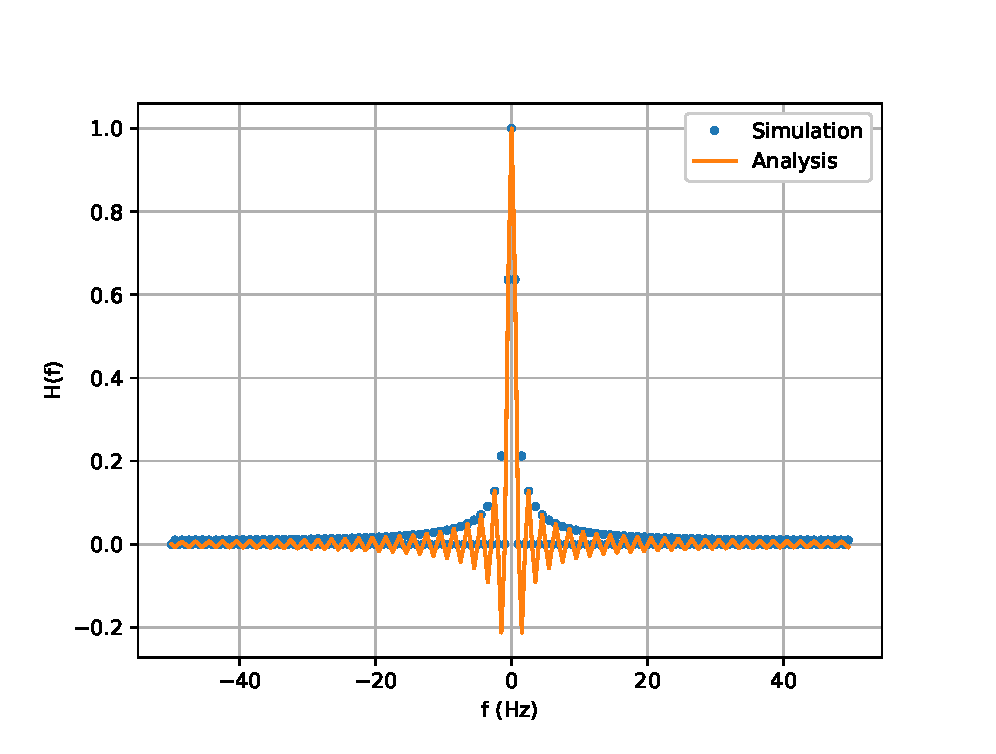
\includegraphics[width=\columnwidth]{./figs/3.9}
			\caption{}
			%\label{fig:ckt}
\end{figure}
 \item 
$	 \sinc{t}\system{F} ?$.  Verify using python.\\
\solution
Using \eqref{eq:rectf}, \eqref{eq:duality} and even property of rect function,
\begin{align}
\label{eq:sinc}
\sinc{t}\system{F}\rect{t}
\end{align}
\begin{lstlisting}
wget https://github.com/LokeshBadisa/EE3900-Linear-Systems-and-Signal-Processing/blob/main/charger/codes/3.10.py
python3 3.10.py
 \end{lstlisting}
  \begin{figure}[!ht]
			\centering
			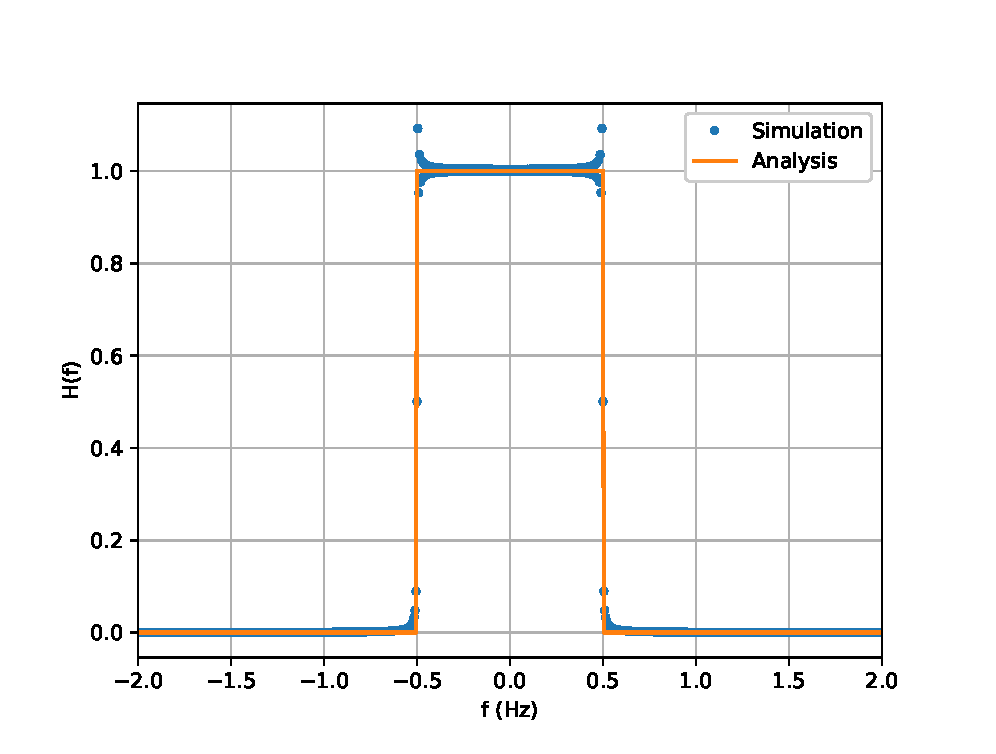
\includegraphics[width=\columnwidth]{./figs/3.10}
			\caption{}
			%\label{fig:ckt}
\end{figure}
\end{enumerate}
\section{Filter}
\begin{enumerate}[label=\thesection.\arabic*
,ref=\thesection.\theenumi]
\item Find $H(f)$ which transforms $x(t)$ to DC 5V.
\solution
\begin{figure}[!ht]
\centering
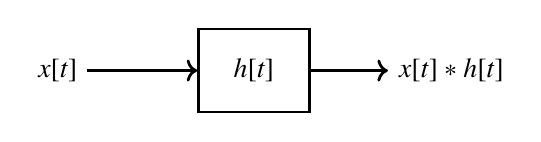
\begin{tikzpicture}
\tikzstyle{block} = [draw, shape=rectangle, minimum height=3em, minimum width=4em, node distance=2cm, line width=1pt]
\node at (-2.5,0) (input) {$x[t]$};
\node [block] (h) {$h[t]$};
\node at (2.5,0) (output) {$x[t]*h[t]$};
\begin{scope}[line width=1pt]
         \draw[->] (input) -- (h);
         \draw[->] (h) -- (output); 
    \end{scope}
\end{tikzpicture}
\end{figure}
\begin{figure}[!ht]
\centering
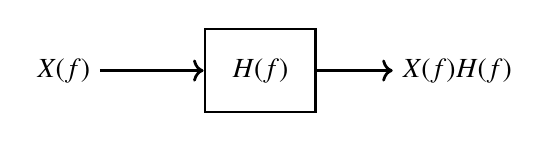
\begin{tikzpicture}
\tikzstyle{block} = [draw, shape=rectangle, minimum height=3em, minimum width=4em, node distance=2cm, line width=1pt]
\node at (-2.5,0) (input) {$X(f)$};
\node [block] (h) {$H(f)$};
\node at (2.5,0) (output) {$X(f)H(f)$};
\begin{scope}[line width=1pt]
         \draw[->] (input) -- (h);
         \draw[->] (h) -- (output); 
    \end{scope}
\end{tikzpicture}
\end{figure}
\begin{align}
X(f)H(f)=V_0\delta(f)
\end{align}
Above equation indicates that H(f) will pass X(f) for f=0.\\
\,$\therefore$ H(f) should be a low pass filter.
\begin{align}
|H(f)|=\frac{V_0}{\brak{\frac{2A_0}{\pi}}}=\frac{V_0\pi}{2A_0}\\
H(f)=\frac{V_0\pi}{2A_0} \hspace{10pt}in\hspace{8pt}-2f_0\leq f\leq 2f_0\\
\label{eq:hf}
H(f)=\frac{V_0\pi}{2A_0}\rect{\frac{f}{4f_0}}
\end{align}
\item Find $h(t)$.\\
\solution 
Using \eqref{eq:hf} and \eqref{eq:sinc},
\begin{align}
h(t)=\frac{2V_0\pi f_0}{A_0}\sinc{4f_0t}
\end{align}
\item Verify your result using  through convolution.
\solution
\begin{lstlisting}
wget https://github.com/LokeshBadisa/EE3900-Linear-Systems-and-Signal-Processing/blob/main/charger/codes/4.3.py
python3 4.3.py
 \end{lstlisting}
  \begin{figure}[!ht]
			\centering
			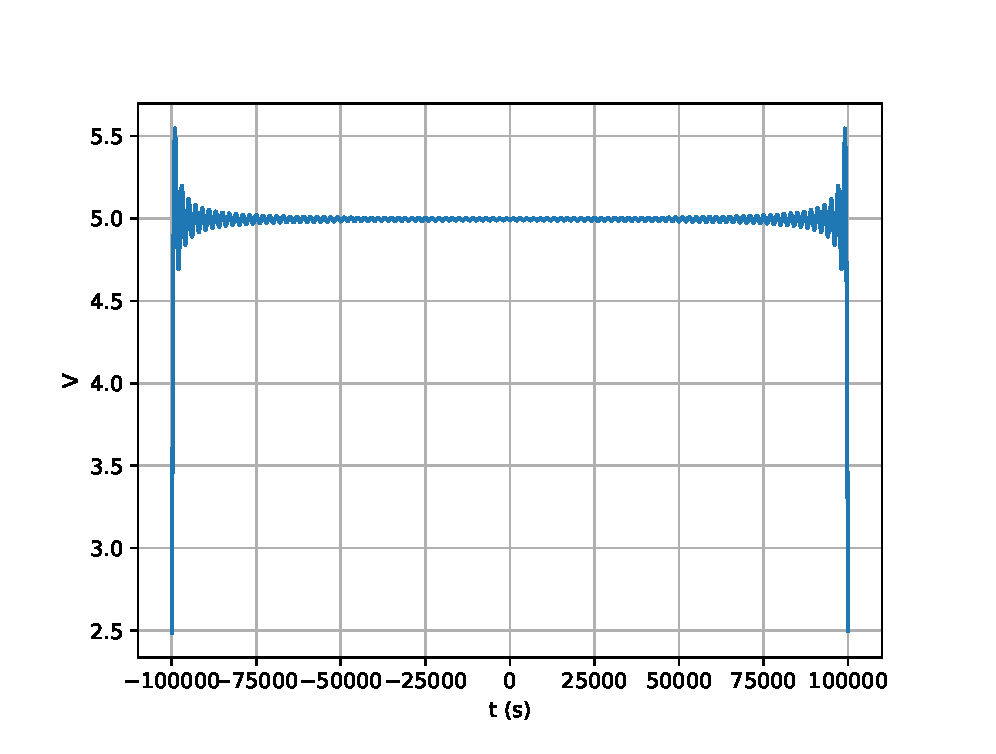
\includegraphics[width=\columnwidth]{./figs/4.3}
			\caption{}
			%\label{fig:ckt}
\end{figure}
\end{enumerate}
\section{Filter Design}
\begin{enumerate}[label=\thesection.\arabic*
,ref=\thesection.\theenumi]
\item Design a Butterworth filter for $H(f)$.\\
\solution The Butterworth filter has an amplitude response
given by
\begin{align}
    \abs{H\brak{f}}^2 = \frac{1}{\brak{1 + \brak{\frac{f}{f_c}}^{2n}}}
\end{align}
where $n$ is the order of the filter and $f_c$ is the cutoff
frequency. The attenuation at frequency $f$ is given by 
\begin{align}
    A &= -10\log_{10}\abs{H\brak{f}}^2 \\
      &= -20\log_{10}\abs{H\brak{f}}
    \label{eq:loss}
\end{align}
We consider the following design parameters for our
lowpass analog Butterworth filter:
\begin{enumerate}
    \item Passband edge, $f_p = 50$ Hz
    \item Stopband edge, $f_s = 100$ Hz
    \item Passband attenuation, $A_p = -1$ dB
    \item Stopband attenuation, $A_s = -20$ dB
\end{enumerate}
We are required to find a desirable order $n$ and cutoff
frequency $f_c$ for the filter. From \eqref{eq:loss},
\begin{align}
    A_p &= -10\log_{10}\sbrak{1 + \brak{\frac{f_p}{f_c}}^{2n}} \\
    A_s &= -10\log_{10}\sbrak{1 + \brak{\frac{f_s}{f_c}}^{2n}}
\end{align}
Thus,
\begin{align}
    \brak{\frac{f_p}{f_c}}^{2n} = 10^{-\frac{A_p}{10}} - 1 \label{eq:fc1} \\
    \brak{\frac{f_s}{f_c}}^{2n} = 10^{-\frac{A_s}{10}} - 1 \label{eq:fc2}
\end{align}
Therefore, on dividing the above equations and solving for $n$,
\begin{align}
    n = \frac{\log\brak{10^{-\frac{A_s}{10}} - 1} - 
    \log\brak{10^{-\frac{A_p}{10}} - 1}}{2\brak{\log{f_s} - \log{f_p}}}
\end{align}
In this case, making appropriate susbstitutions gives $n = 4.29$.
Hence, we take $n = 5$. Solving for $f_c$ in \eqref{eq:fc1} and
\eqref{eq:fc2},
\begin{align}
    f_{c1} = f_p\sbrak{10^{-\frac{A_p}{10}} - 1}^{-\frac{1}{2n}} = \SI[parse-numbers=false]{57.23}{\hertz} \\
    f_{c2} = f_s\sbrak{10^{-\frac{A_s}{10}} - 1}^{-\frac{1}{2n}} = \SI[parse-numbers=false]{63.16}{\hertz}
\end{align}
Hence, we take $f_c = \sqrt{f_{c1}f_{c2}} = \SI[parse-numbers=false]{60}{\hertz}$ approximately.
\item Design a Chebyshev filter for $H(f)$.
\solution The Chebyshev filter has an amplitude response
given by
\begin{align}
    \abs{H\brak{f}}^2 = \frac{1}{\brak{1 + \epsilon^2C_n^2\brak{\frac{f}{f_c}}}}
\end{align}
where 
\begin{enumerate}
    \item $n$ is the order of the filter
    \item $\epsilon$ is the ripple
    \item $f_c$ is the cutoff frequency 
    \item $C_n = \cosh^{-1}\brak{n\cosh{x}}$ denotes 
    the n\textsuperscript{th} order Chebyshev polynomial,
    given by
    \begin{align}
        c_n(x) =
        \begin{cases}
            \cos\brak{n\cos^{-1}x} & \abs{x} \le 1 \\
            \cosh\brak{n\cosh^{-1}x} & \textrm{otherwise}
        \end{cases}
        \label{eq:chebypol}
    \end{align}
\end{enumerate}
We are given the following specifications:
\begin{enumerate}
    \item Passband edge (which is equal to 
    cutoff frequency), $f_p = f_c$
    \item Stopband edge, $f_s$
    \item Attenuation at stopband edge, $A_s$
    \item Peak-to-peak ripple $\delta$ in the passband.
    It is given in dB and is related to $\epsilon$ as
    \begin{align}
        \delta = 10\log_{10}\brak{1 + \epsilon^2}
        \label{eq:delta-eps}
    \end{align}
\end{enumerate}
and we must find a suitable $n$ and $\epsilon$. From
\eqref{eq:delta-eps},
\begin{align}
    \epsilon = \sqrt{10^{\frac{\delta}{10}} - 1}
    \label{eq:epsilon-del}
\end{align}
At $f_s > f_p = f_c$, using \eqref{eq:chebypol}, $A_s$ is given by
\begin{align}
    A_s = -10\log_{10}\sbrak{1 + \epsilon^2c_n^2\brak{\frac{f_s}{f_p}}} \\
    \implies c_n\brak{\frac{f_s}{f_p}} = \frac{\sqrt{10^{-\frac{A_s}{10}} - 1}}{\epsilon} \\
    \implies n = \frac{\cosh^{-1}\brak{\frac{\sqrt{10^{-\frac{A_s}{10}} - 1}}{\epsilon}}}
    {\cosh^{-1}\brak{\frac{f_s}{f_p}}}
\end{align}
We consider the following specifications:
\begin{enumerate}
    \item Passband edge/cutoff frequency, $f_p = f_c = \SI[parse-numbers=false]{60}{\hertz}$.
    \item Stopband edge, $f_s = \SI[parse-numbers=false]{100}{\hertz}$.
    \item Passband ripple, $\delta = \SI[parse-numbers=false]{0.5}{\dB}$
    \item Stopband attenuation, $A_s = \SI[parse-numbers=false]{-20}{\dB}$
\end{enumerate}
$\epsilon = 0.35$ and $n = 3.68$. Hence, we take $n = 4$
as the order of the Chebyshev filter.
\item Design a circuit for your Butterworth filter.
\solution Looking at the table of normalized element values
$L_k$, $C_k$, of the Butterworth filter for order 5, and noting
that de-normalized values $L_k'$ and $C_k'$ are given by
\begin{align}
    C_k' = \frac{C_k}{\omega_c} \qquad L_k' = \frac{L_k}{\omega_c}
\end{align}
De-normalizing these values, taking $f_c = 60$ Hz,
\begin{align}
    C_1' = C_5' = \SI{1.64}{\milli\farad} \\
    L_2' = L_4' = \SI{4.29}{\milli\henry} \\
    C_3' = \SI{5.31}{\milli\farad} \\
\end{align}
The L-C network is shown in Fig. \ref{fig:butter-filter}.
\begin{figure}[!ht]
    \centering
    \begin{circuitikz} 
        \draw (0,0) to[short, o-o] (7,0);
        \draw (0,2) to [short, o-] (1,2) to [L, l=4.29 mH] (3.5,2) to [L, l=4.29 mH] (6,2) to[short, -o] (7,2);
        \draw (1,0) to[C, l=1.64 mF] (1,2);
        \draw (3.5,0) to[C, l=5.31 mF] (3.5,2);
        \draw (6,0) to[C, l=1.64 mF] (6,2);
    \end{circuitikz}
    \caption{L-C Butterworth Filter}
    \label{fig:butter-filter}
\end{figure}
This circuit is simulated in the ngspice code \texttt{codes/5\_3.cir}.
The Python code \texttt{codes/5\_3.py} compares the amplitude response
of the simulated circuit with the theoretical expression.
\item Design a circuit for your Chebyshev filter.
%\begin{figure}
 %   \includegraphics[width=\columnwidth]{figs/5.3}
  %  \caption{Simulation of Butterworth filter.}
   % \label{fig:sim-butter}
%\end{figure}
\solution Looking at the table of normalized element values
of the Chebyshev filter for order 3 and 0.5 dB ripple,
and de-nomrmalizing those values, taking $f_c = \SI[parse-numbers=false]{50}{\hertz}$,
\begin{align}
    C_1' = \SI{4.43}{\milli\farad} \\
    L_2' = \SI{3.16}{\milli\henry} \\
    C_3' = \SI{6.28}{\milli\farad} \\
    L_4' = \SI{2.23}{\milli\henry}
\end{align}
The L-C network is shown in Fig. \ref{fig:cheby-filter}.
\begin{figure}[!ht]
    \centering
    \begin{circuitikz} 
        \draw (0,0) to[short, o-o] (7,0); 
        \draw (1,0) to[C, l=4.43 mF] (1,2);
        \draw (3.5,0) to[C, l=6.28 mF] (3.5,2);
        \draw (0,2) to [short, o-] (1,2) to [L, l=3.16 mH] (3.5,2) to[L, l=2.23 mH] (6,2) to[short, -o] (7,2);
    \end{circuitikz}
    \caption{L-C Chebyshev Filter}
    \label{fig:cheby-filter}
\end{figure}
This circuit is simulated in the ngspice code \texttt{codes/5\_4.cir}.
The Python code \texttt{codes/5\_4.py} compares the amplitude response
of the simulated circuit with the theoretical expression.
\begin{figure}
    \includegraphics[width=\columnwidth]{figs/original}
    \caption{Simulation of Chebyshev filter.}
    \label{fig:sim-cheby}
\end{figure}
\end{enumerate}
\end{document}
